\documentclass[a4paper]{scrreprt}
\usepackage[T1]{fontenc}
\usepackage[utf8]{inputenc}
\usepackage[ngerman]{babel}
\usepackage{graphicx}
\usepackage{subfigure}
\usepackage[official]{eurosym}
\begin{document}
\author{Josephine Reiche}
\title{Mathematische Grundlagen des Machine-/ Deep Learning}
\maketitle
\tableofcontents
\chapter{Selbstständigkeitserklärung}
Der Arbeit ist folgende Erklärung beizufügen:
Hiermit versichere ich, dass ich die schriftliche Hausarbeit selbstständig verfasst und keine
anderen als die angegebenen Quellen und Hilfsmittel benutzt habe. Die Stellen meiner Arbeit,
die dem Wortlaut oder dem Sinne nach anderen Werken und Quellen, einschließlich Quellen
aus dem Internet, entnommen sind, habe ich in jedem Fall unter Angabe der Quelle deutlich
als Entlehnung kenntlich gemacht. Dasselbe gilt sinngemäß für Tabellen, Karten und
Abbildungen.

(Unterschrift)

% !TEX root = Facharbeit_Mathe_Grundlagen_ML-DL.tex
\chapter{Einführung}
In meiner Facharbeit möchte ich mich mit dem Thema „Künstliche Intelligenz“ intensiv auseinandersetzen. Die USA, China und Europa kämpfen um die Vorherrschaft, in diesem neuen Gebiet der Informatik, welche die Zukunft in unserem Leben revolutionieren wird. Doch was bedeutet eigentlich künstliche Intelligenz? Was macht dieses Thema so interessant und Zukunftsrelevant, dass nun sogar Deutschland drei Milliarden Euro investieren möchte? Erstmal ist die Künstliche Intelligenz (KI) ein Teilgebiet der Informatik, die ihren Ursprung im 20. Jahrhundert hatte. Dieses Teilgebiet befasst sich mit maschinellem Lernen und der Automatisierung intelligenten Verhaltens. Schon heute findet man vielseitige Anwendungen von KI. Beispiele dafür sind die Gesichtserkennung, die Google-Sucherkennung und Werbung. Zahlreiche Anwendungsbereiche in Naturwissenschaft, Medizin, Technik, Informatik und im Medienbereich sind möglich. Das spannende an KI, Machine Learning und Deep Learning ist, dass es auf Grundlagen der Mathematik basiert. Das heißt, dass es auch einem Schüler möglich ist, mit dem mathematischen Wissen für die Sekundarstufe II, die Grundzüge der KI nachzuvollziehen. Das motiviert zum einen worin die Mathematik zum Teil ihre praktische Anwendung findet und was man als Schüler leisten kann. 

% !TEX root = Facharbeit_Mathe_Grundlagen_ML-DL.tex
\chapter{Regression}
\section{Lineare Regression}

Im Kontext des Machine Learning ist die lineare Regression den supervised Modellen zuzuordnen, die auf vorgegebenen Eingabe- und Ausgabedaten basieren. Die Ergebnisse der linearen Regression sind diskrete Werte (z.B. Geld, Quadratmeter).\\\\
Defintion: Die lineare Regression ist eine statistische Methode, um die Daten aus einer Stichprobe oder einem Experiment durch eine angenommene lineare Funktion zu beschreiben.
%(https://learnattack.de/mathe/lineare-regression)\\\\
Zur bessern Veranschaulichung der zu Grunde liegenden Prinzipien werden im folgenden Funktionen mit einer Variablen x betrachtet. 
Dabei soll gelten:

X - Menge aller Eingabewerte

Y - Menge aller Ausgabewerte

$x_i$ - \textit{i}tes Element aus X

$y_i$ - \textit{i}tes Element aus Y

n - Anzahl der Elemente von X und Y

f(x)= a+b*x\\\\

Das allgemeine Vorgehen bei der linearen Regression lässt sich durch folgendes Schema darstellen (Abb. x).
\begin{figure}[htbp]
\centering
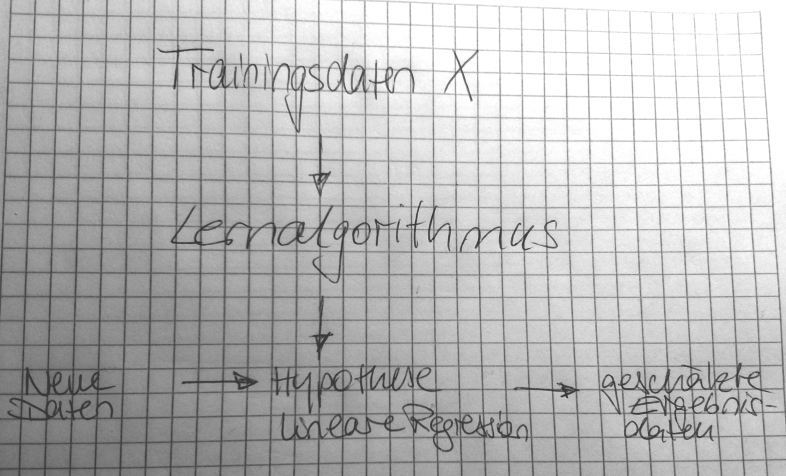
\includegraphics[scale=.2]{Abbildungen/Lineare_Regression/LinRegModell}
\label{Abb:Modell}
\caption{Modell}
\end{figure}

Es gibt mehrere Verfahren diese Funktion zu ermitteln.

\begin{enumerate}
\item Graphische Verfahren

Hier werden die ermittelten Messwerte in einem Koordinatensystem abgebildet. Dies kann mittels eines Geometrieprogramms oder dem Schultaschenrechner durchgeführt werden. Anschließend wird eine lineare Funktion manuell im Koordinatensystem verschoben und die Abstände von den Punkten zu der Funktion nach Augenmaß minimiert. Die Parameter der gewählten linearen Funktion können dann übernommen werden. In den Abbildungen sind die Abstände zwischen den tatsächlichen Punkten und der Funktionsgerade am entsprechenden x-Wert durch grüne Strecken angegeben. Je länger die Strecke, desto größer der Fehler, desto geringer die Eignung der Funktion als Modell. Die folgende Abbildung zeigt eine ungünstige und eine perfekte grafische Lösung des Modells.

\begin{figure}[htbp]
\centering
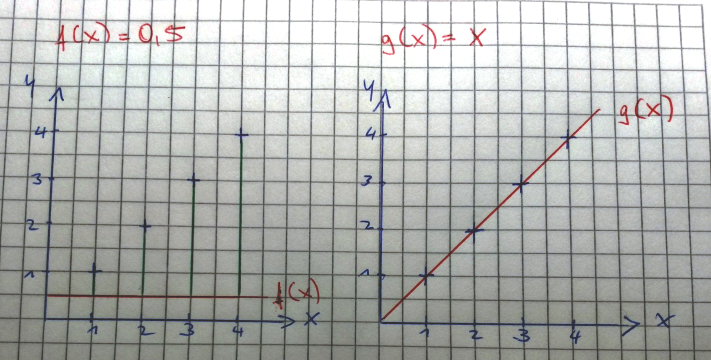
\includegraphics[scale=.5]{Abbildungen/Lineare_Regression/GrafikVerfahren}
\label{Abb:Lösungen}
\caption{Lösungen}
\end{figure}


\item Manuelle Berechnungen

Die lineare Regression kann, besonders bei überschaubarer Anzahl von Datensätzen (n), händisch bestimmt werden. Zunächst wird der Korrelationskoeffizient r, mit der Formel:


$r= \frac{\sum (x_i-\bar{x})*(y_i-\bar{y})}{\sqrt{\sum (x_i-\bar{x})^{2}*(y_i-\bar{y})^{2}}}$,


wobei $\bar{x}$ (entsprechend $\bar{y}$) das arithmetische Mittel nach $\frac{1}{n}*\sum_{i=1}^{n} x_i$
ist, berechnet.



Danach wird die Steigung b  der linearen Funktion ermittelt:

$b= r*\frac{S_{y}}{S_{x}}$

Diese Formel enthält die Standardabweichung von y und x, die wie folgt bestimmt werden:

$S_{y}= \sqrt{\frac{\sum (y-\bar{y})^{2}}{n-1}}$

$S_{x}= \sqrt{\frac{\sum (x-\bar{x})^{2}}{n-1}}$

Zuletzt wird die Verschiebungskonstante a durch einfaches Umstellen berechnet: 
%Verschiebungskonstante alternative Bezeichnung ist Ordinatenabschnitt oder y-Achsenabschnitt?

$a=\bar{y}-b*\bar{x}$

Somit sind alle Parameter für die Funktion $y=a+b*x$ bestimmt. \\\\
Die folgende Tabelle enthält Beispieldaten für den Verkaufspreis einer Wohnung, der hier nur von der Wohnungsgröße in $m^{2}$ abhängt.



\begin{table}
\centering
\refstepcounter{table}
\label{Manuelle Regression}
\begin{tabular}{lllllll}
\textbf{A in $m^{2}$} & \textbf{Preis in \euro{} } & $x_i-\bar{x}$ & $y_i-\bar{y}$ & $(x_i-\bar{x})*(y_i-\bar{y})$ & $(x_i-\bar{x})^{2}$ & $(y_i-\bar{y})^{2}$  \\
70                    & 351000                 & 70                  & 351000              & 24570000                                    & 4900                    & 1,23201E+11             \\
72                    & 390000                 & 72                  & 390000              & 28080000                                    & 5184                    & 1,521E+11               \\
91                    & 473000                 & 91                  & 473000              & 43043000                                    & 8281                    & 2,23729E+11             \\
58                    & 282000                 & 58                  & 282000              & 16356000                                    & 3364                    & 79524000000             \\
49                    & 300000                 & 49                  & 300000              & 14700000                                    & 2401                    & 90000000000             \\
50                    & 286000                 & 50                  & 286000              & 14300000                                    & 2500                    & 81796000000             \\
48                    & 228000                 & 48                  & 228000              & 10944000                                    & 2304                    & 51984000000             \\
33                    & 181000                 & 33                  & 181000              & 5973000                                     & 1089                    & 32761000000             \\
61                    & 308000                 & 61                  & 308000              & 18788000                                    & 3721                    & 94864000000             \\
51                    & 289000                 & 51                  & 289000              & 14739000                                    & 2601                    & 83521000000             \\
78                    & 414000                 & 78                  & 414000              & 32292000                                    & 6084                    & 1,71396E+11             \\
70                    & 358000                 & 70                  & 358000              & 25060000                                    & 4900                    & 1,28164E+11             \\
35                    & 165000                 & 35                  & 165000              & 5775000                                     & 1225                    & 27225000000             \\
81                    & 397000                 & 81                  & 397000              & 32157000                                    & 6561                    & 1,57609E+11             \\
70                    & 352000                 & 70                  & 352000              & 24640000                                    & 4900                    & 1,23904E+11             \\
47                    & 239000                 & 47                  & 239000              & 11233000                                    & 2209                    & 57121000000             \\
55                    & 322000                 & 55                  & 322000              & 17710000                                    & 3025                    & 1,03684E+11             \\
70                    & 376000                 & 70                  & 376000              & 26320000                                    & 4900                    & 1,41376E+11             \\
89                    & 499000                 & 89                  & 499000              & 44411000                                    & 7921                    & 2,49001E+11             \\
68                    & 383000                 & 68                  & 383000              & 26044000                                    & 4624                    & 1,46689E+11             \\
42                    & 229000                 & 42                  & 229000              & 9618000                                     & 1764                    & 52441000000             \\
93                    & 424000                 & 93                  & 424000              & 39432000                                    & 8649                    & 1,79776E+11             \\
54                    & 256000                 & 54                  & 256000              & 13824000                                    & 2916                    & 65536000000             \\
52                    & 256000                 & 52                  & 256000              & 13312000                                    & 2704                    & 65536000000             \\
72                    & 363000                 & 72                  & 363000              & 26136000                                    & 5184                    & 1,31769E+11             \\
62                    & 328000                 & 62                  & 328000              & 20336000                                    & 3844                    & 1,07584E+11             \\
65                    & 331000                 & 65                  & 331000              & 21515000                                    & 4225                    & 1,09561E+11             \\
98                    & 465000                 & 98                  & 465000              & 45570000                                    & 9604                    & 2,16225E+11             \\
39                    & 273000                 & 39                  & 273000              & 10647000                                    & 1521                    & 74529000000             \\
50                    & 215000                 & 50                  & 215000              & 10750000                                    & 2500                    & 46225000000             \\
62                    & 287000                 & 62                  & 287000              & 17794000                                    & 3844                    & 82369000000             \\
45                    & 207000                 & 45                  & 207000              & 9315000                                     & 2025                    & 42849000000             \\
11                    & 7000                   & 11                  & 7000                & 77000                                       & 121                     & 49000000                \\
60                    & 328000                 & 60                  & 328000              & 19680000                                    & 3600                    & 1,07584E+11             \\
60                    & 282000                 & 60                  & 282000              & 16920000                                    & 3600                    & 79524000000             \\
74                    & 322000                 & 74                  & 322000              & 23828000                                    & 5476                    & 1,03684E+11             \\
64                    & 305000                 & 64                  & 305000              & 19520000                                    & 4096                    & 93025000000             \\
56                    & 317000                 & 56                  & 317000              & 17752000                                    & 3136                    & 1,00489E+11             \\
71                    & 406000                 & 71                  & 406000              & 28826000                                    & 5041                    & 1,64836E+11             \\
40                    & 225000                 & 40                  & 225000              & 9000000                                     & 1600                    & 50625000000             \\
76                    & 407000                 & 76                  & 407000              & 30932000                                    & 5776                    & 1,65649E+11             \\
88                    & 443000                 & 88                  & 443000              & 38984000                                    & 7744                    & 1,96249E+11             \\
55                    & 294000                 & 55                  & 294000              & 16170000                                    & 3025                    & 86436000000             \\
60                    & 277000                 & 60                  & 277000              & 16620000                                    & 3600                    & 76729000000             \\
79                    & 393000                 & 79                  & 393000              & 31047000                                    & 6241                    & 1,54449E+11             \\
109                   & 576000                 & 109                 & 576000              & 62784000                                    & 11881                   & 3,31776E+11             \\
51                    & 254000                 & 51                  & 254000              & 12954000                                    & 2601                    & 64516000000             \\
48                    & 263000                 & 48                  & 263000              & 12624000                                    & 2304                    & 69169000000             \\
25                    & 101000                 & 25                  & 101000              & 2525000                                     & 625                     & 10201000000             \\
88                    & 426000                 & 88                  & 426000              & 37488000                                    & 7744                    & 1,81476E+11             \\
61,9                  & 317060                 &                     &                     & 1073115000                                  & 209685                  & 5,53052E+12            
\end{tabular}
\end{table}

Aus der Tabelle lassen sich folgende Werte berechnen:

$\bar{x}$= 61,9
$\bar{y}$= 317060 

$r= \frac{1073115000}{\sqrt{209685*5,53052E+12}}=0,961018288$

$S_{y}= \sqrt{\frac{5,04163 E+11}{50-1}}=101434,8912$

$S_{x}= \sqrt{\frac{18104,5}{50-1}}=19,22185194$

$b= 0,961018288*\frac{101434,8912}{19,22185194}=5071,352426$
 
$a=317060-5071,352426*61,9=3143,284819$

Der Anstieg der durch die Regression ermittelten Funktion beträgt 5071,352426 und die Verschiebungskonstante ist 3143,284819.

%Hier ein Beispiel eintragen für Training und Vorraussage.

\item Algorithmische Berechnung

Die vorgestellte Methode der Berechnung der Funktionsparameter ist nur für kleinere Datensätze und wenige, hier eine abhängige Variable (x) praktikabel. In der Praxis werden jedoch möglichst große Datenmengen mit hunderten oder tausenden Abhängigen verwendet, deren Parameter bestimmt werden sollen. Dazu ist ein algorithmisches Vorgehen notwendig, das hier anhand des einfachen bereits eingeführten Beispiels erläutert wird.\\\\
Dabei werden die in vielen Bereichen des ML/DL genutzten Verfahren Gradientenabstieg (gradient-descent), die Kostenfunktion und die Lernrate eingeführt. 

\textbf {Kostenfunktion (Cost function)}

Die Kostenfunktion gibt ein Maß an, das die Fähigkeit des Modells, die Relation zwischen X und Y zu bestimmen, beschreibt. 

Mathematisch formuliert:

$J (a,b)=\frac{1}{n}\sum_{i=0}^{n} (y_i-(a+b*x_i))^{2}$ 
%https://ml-cheatsheet.readthedocs.io/en/latest/linear_regression.html#cost-function
%Quelle gibt N im Bruch statt n an? Habe mich erstmal für den n entschieden.

%Gute Erklärung https://math.stackexchange.com/questions/2433022/the-cost-function-derivation-in-andrew-ng-machine-learning-course

wobei $(a+b*x_i)$ die Vorhersage für den Wert an der Stelle $x_i$ und $y_i$ der tatsächliche Wert für $x_i$ ist. Die Differenz ist der Abstand beziehungsweise der Fehler der Regressionsgeraden bezüglich $y_i$. Zur Berechnung des Fehlers (Kosten) können verschiedene Abstandsnormen angewendet werden. Hier wird der Euklidische Abstand angewendet, unter anderem um negative Ergebnisse für den Fehler auszuschließen und die Funktion differenzierbar zu machen.
 %weitere Erkenntnis: Udemy Intuition Geogebra Beispiel Konstante Funktion, nicht quadrierte Abstände führen zu beliebig vielen Lösungen, möglicherweise keine Ableitung möglich? Kein Minimum? 
Die ermittelten Fehler werden summiert und durch die Anzahl der Datensätze geteilt, wodurch der mittlere Fehler (mittlerer Abstand) berechnet wird. Ziel ist es, den mittlere Fehler und somit die Kostenfunktion $J(a,b)$ zu minimieren.
%Hier Pythonquellcode für diese Berechnungen einfügen

\textbf {Gradientenabstiegsverfahren (Gradient descent)}

Die Minimierung der Kostenfunktion $J(a,b)$ ist ein Optimierungsproblem, das durch Nullsetzen der ersten Ableitung gelöst wird. Das Nullsetzen der Ableitung ist für übliche Datenmengen nur durch numerische Verfahren effizient lösbar. Mögliche Ergebnisse dieser Verfahren können jedoch  auch lokale/globale Minima oder Maxima sein. Folgende Intuition zeigt das ausschließliche Vorhandensein eines globalen Minimums für die hier betrachteten Funktionen mit einer Variablen $x$. Zunächst wird der Parameter $a=0$ gesetzt, womit nur noch lineare Funktionen durch den Koordinatenursprung $f(x)=b*x$ möglich sind. 
Angenommen die korrekte Funktion entspricht $f(x)=x$ mit b=1. In der folgenden Abbildung sind mögliche Funktionen mit weiteren Werten $b=\{0; 0,5; 1; 1,5; 2\}$ eingetragen. Die Ergebnisse der Kostenfunktionen für die verschiedenen $b$ in Abbildung (c) zeigen, dass für die Werte $J(b)$ eine Parabel entsteht.  

\begin{figure}[htbp]
\centering
\subfigure[Funktionen a=0]{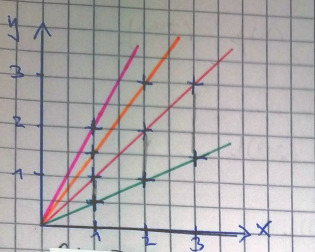
\includegraphics[scale=.5]{Abbildungen/Lineare_Regression/Gradientenabstiegsverfahren1}}
\subfigure[f(b)]{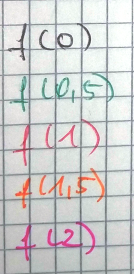
\includegraphics[scale=.5]{Abbildungen/Lineare_Regression/Gradientenabstiegsverfahren3}}
\subfigure[J(b)]{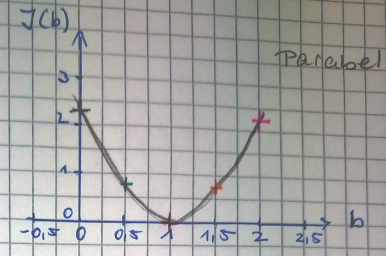
\includegraphics[scale=.5]{Abbildungen/Lineare_Regression/Gradientenabstiegsverfahren2}}
\label{Abb:Lösungen}
\caption{Intuition Kostenfunktion}
\end{figure}
Die Ableitung $J'(b)=0$ gilt für $b=1$, was in diesem Beispiel exakt dem Minimum der Funktion entspricht. Wird der Parameter $a$ hinzugezogen, ergibt sich statt einer Parabel eine konvexe Funktion.

\begin{figure}[htbp]
\centering
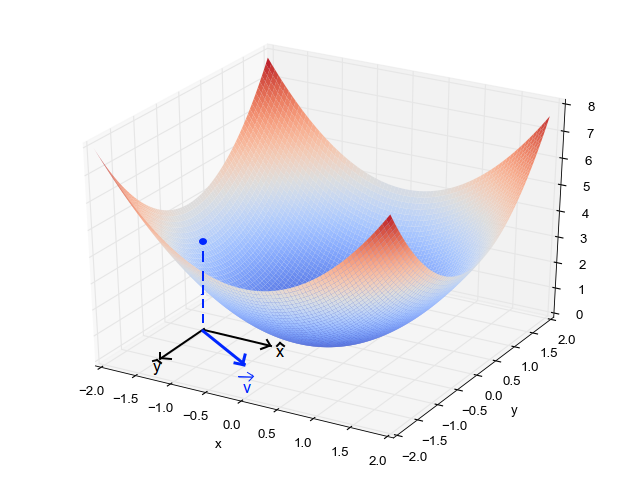
\includegraphics[scale=.5]{Abbildungen/Lineare_Regression/konvexe_funktion}
\label{Abb:konvexe Funktion}
\caption{konvexe Funktion}
\end{figure}


Auch diese hat ein globales Minimum. Demnach ist die Kostenfunktion nach  a und b partiell zu differenzieren, um das Minimum zu berechnen. Dafür wird die Kostenfunktion um die Konstante 2 erweitert, was die Berechnung der Ableitung erleichtert.

$J (a,b)=\frac{1}{2*n}\sum_{i=1}^{n} (y_i-(a+b*x_i))^{2}$ 
  
Demzufolge ergeben sich folgende innere Ableitungen für $f_{a,b}(x_i)$ nach jeweils $a$ und $b$:
\\\\
$f_{a,b}(x_i)=a+b*x_i$
\\\\
$J (a,b)= \frac{1}{2*n}\sum_{i=1}^{n} (y_i-(a+b*x_i))^{2}$
\\\\
$\frac{\Delta}{\Delta a} f_{a,b} (x_i)= \frac{\Delta}{\Delta a} (a+b*x_i)=\frac{\Delta}{\Delta a} a+\frac{\Delta}{\Delta a} b*x_i=1+0=1$
\\\\
$\frac{\Delta}{\Delta b} f_{a,b} (x_i)= \frac{\Delta}{\Delta b} (a+b*x_i)=\frac{\Delta}{\Delta b}+a+\frac{\Delta}{\Delta b}bx_i=0+x_i =x_i$
\\\\
Die äußere Ableitung ist:

$J`_{(a,b)} (x_i)=\frac{1}{2*n}\sum_{i=1}^{n} 2 (f_{a,b}(x_i)-y_i)= \frac{1}{n}\sum_{i=1}^{n}  (f_{a,b}(x_i)-y_i)$
\\\\
Die partielle Ableitung von $J (a,b)$ ergibt nach der Kettenregel für $a$ und $b$ folgende Terme:
\\\\
$\frac{\Delta}{\Delta a} J(a,b)= \frac{1}{n}\sum_{i=1}^{n} (f_{a,b} (x_i)-y_i)$
\\\\
$\frac{\Delta}{\Delta b} J(a,b)= \frac{1}{n}\sum_{i=1}^{n} (f_{a,b} (x_i)-y_i)*x_i$
\\\\
% Bild Anstieg $a$ und $b$ Richtung neuer Wert
Nachdem die Grundlagen des Verfahrens beschrieben sind, sind die einzelnen Berechnungen zu einem Algorithmus zusammenzufassen. Zunächst werden für die Parameter $a$ und $b$ zufällige Werte gewählt. Dann wird für alle $x_i$-Werte die Fehlerfunktion ausgerechnet. Die Anstiege von $a$ und $b$ geben per Vorzeichen die Richtung an, in welcher der Folgewert für $a$ und $b$ gewählt wird. Das Ziel ist, das globale Minimum der Fehlerfunktion zu ermitteln. Dazu muss ein Konvergenzkriterium bestimmt werden. Das Konvergenzkriterium kann verschieden definiert werden. In vielen Fällen wird der Algorithmus über eine vorgegebene Anzahl von Iterationen ausgeführt. Andere Algorithmen vergleichen die Änderungen der Werte der Fehlerfunktion und brechen bei Unterschreiten eines vorgegebenen Mindestdeltas ab. Die Größe der Änderung pro Iteration wird durch einen Hyperparameter, der Lernrate $\alpha$, bestimmt. Die Zuweisung der neuen Werte wird durch das Zeichen $:=$ dargestellt. Daraus folgt:

$a:= a - \alpha * \frac{\Delta}{\Delta a} J(a,b)$
\\\\
$b:= b - \alpha * \frac{\Delta}{\Delta b} J(a,b)$

Das Gradient Descent Verfahren ist ein allgemeine Konzept, das in vielen Bereichen Anwendung findet. Je nach Anwendung kann auch das Gradient Descent Verfahren optimiert werden. Für stabile Funktionen und wenige Testdaten, wie in diesem Beispiel, ist das \textbf{Batch-Gradient-Descent} Verfahren geeignet. Dabei wird die Summe der Fehlerfunktion über alle Testdatensätze berechnet und eine stabiler Wert führt zum Update und damit zu einer stabilen Konvergenz des Abstiegs.
\\\\
Das \textbf{Stochastic-Gradient-Descent} Verfahren führt ein Update der Parameter nach jedem einzelnen Datensatz durch. Abhängig von der Anwendung kann dies schneller zur Konvergenz führen. In vielen Fällen kann es aber dazu führen, das die Fehlerfunktion stark variiert und nicht mehr konvergiert. Dieses Verfahren benötigt einen höheren Rechenaufwand als das vorgenannte.
\\\\
In vielen Anwendungen wird eine Kombination aus den beiden beschriebenen Verfahren, das \textbf{Mini-Batch-Gradient-Descent} Verfahren gebildet.
Dabei wird das SGD auf kleinere Mengen des Datensatze den Minibatches, z.B. auf 256 Datensätze gleichzeitig, angewendet. Die Vorteile der beiden Verfahren werden somit kombiniert. 
    

\end{enumerate}

 



\end{document}



